\documentclass[tikz,svgnames]{standalone}

\usetikzlibrary{mindmap}

\begin{document}

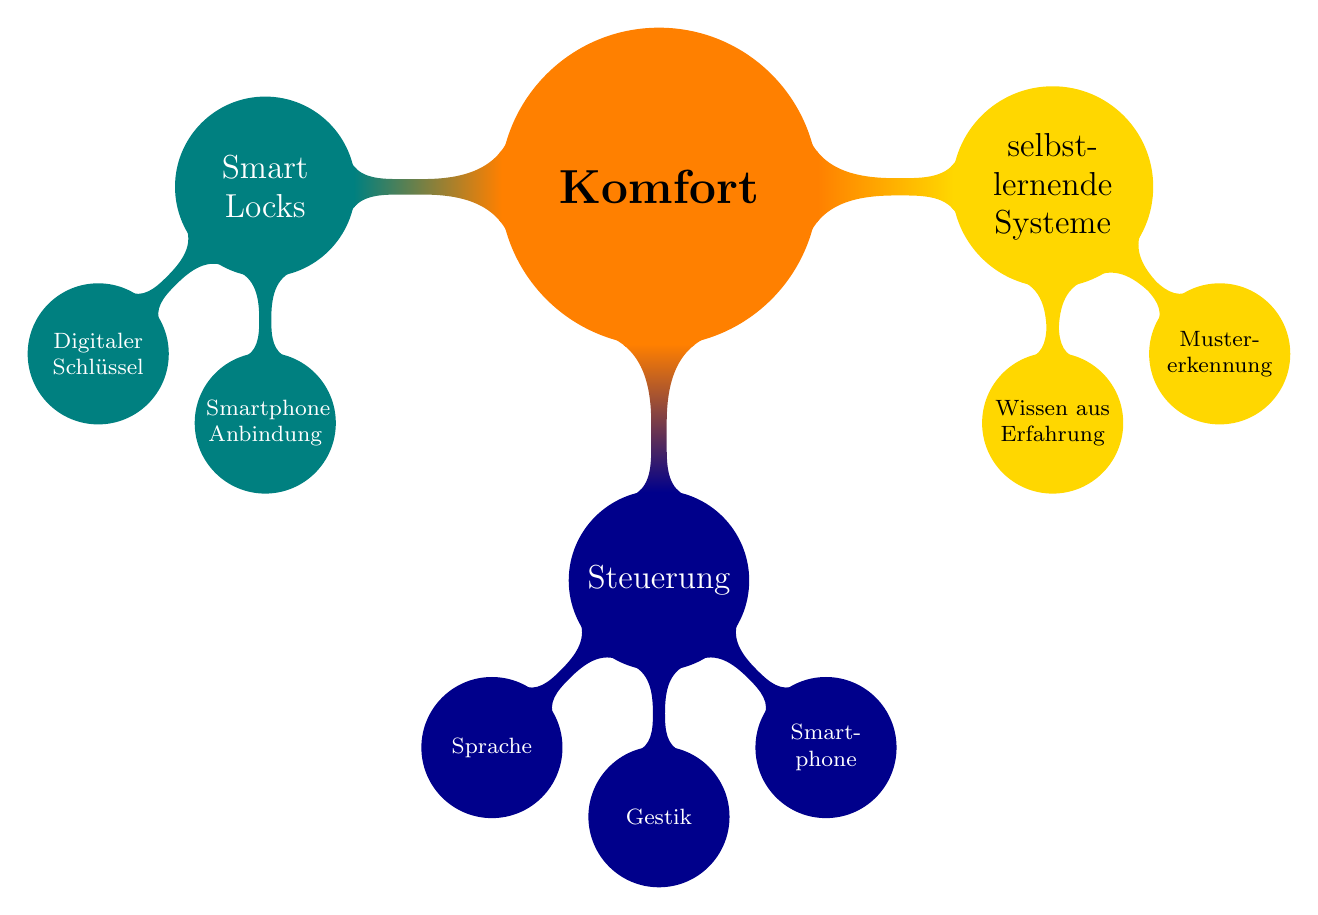
\begin{tikzpicture}[
    mindmap, grow cyclic, every node/.style=concept, concept color=orange,
    level 1/.append style={level distance=5cm,sibling angle=90,font=\large},
    level 2/.append style={level distance=3cm,sibling angle=45}
  ]

  \node{\textbf{\LARGE{Komfort}}} [clockwise from=0]
  child [concept color=Gold] { node {selbst\-lernende Systeme} [counterclockwise from=270]
      child { node {Wissen aus Erfahrung}}
      child { node {Muster\-erkennung}}
    }
  child [concept color=DarkBlue,text=white] { node {Steuerung} [clockwise from=315]
      child { node {Smart\-phone}}
      child { node {Gestik}}
      child { node {Sprache}}
    }
  child [concept color=teal,text=white] { node {Smart Locks} [clockwise from=270]
      child { node {Smartphone Anbindung}}
      child { node {Digitaler Schlüssel}}
    };
\end{tikzpicture}

\end{document}
